\chapter{Portable Executable Format} \label{chap:peformat}

The \PE{} is a file format for executables and object files used by Microsoft products. Some examples for \PE{} file types are \DLL{}, \FON{}, \DRV{}, \SYS{} and \EXE{} files.

PortEx extracts the information from the \PE{} format to assist in analysing malware. Therefore knowledge about the \PE{} format is neccessary to understand the inner workings of the library PortEx.

The \PE{} format is described in the \emph{Microsoft Portable Executable and Common Object File Format Specification} \cite{pespec}

\section{General Structure}

Figure~\ref{fig:peformat} illustrates the structure of a \PE{} file. An executable \PE{} file always starts with the MS-DOS Stub. This is an application which is able to run in MS-DOS. The standard MS-DOS stub prints the message \enquote{This program cannot be run in DOS mode} and closes right after. 

To determine if a file is of a certain file format, signatures are used. The file format signature is usually at the very beginning of the file. Since the \PE{} starts with the MS-DOS stub, which has a file signature itself, the \PE{} signature is placed after. \todo{MZ, PE00} The offset to the \PE{} signature is defined in location 0x3c of the stub, thus enables Windows to properly execute the \PE{} file. 

Right after the signature follow the COFF File Header, the Optional Header and the Section Table. The COFF File Header contains information about the type of the target machine, the number of sections, a time date stamp that indicates when the file was created, the size of the Optional Header.and flags that indicate file characteristics.

Despite its name the Optional Header is mandatory for image files. Only object files don't need it.

The Section Table describes \ia{} characteristics, size, name and location of the sections that make up the rest of the \PE{} file.

\todo{make your own picture}
\begin{figure}
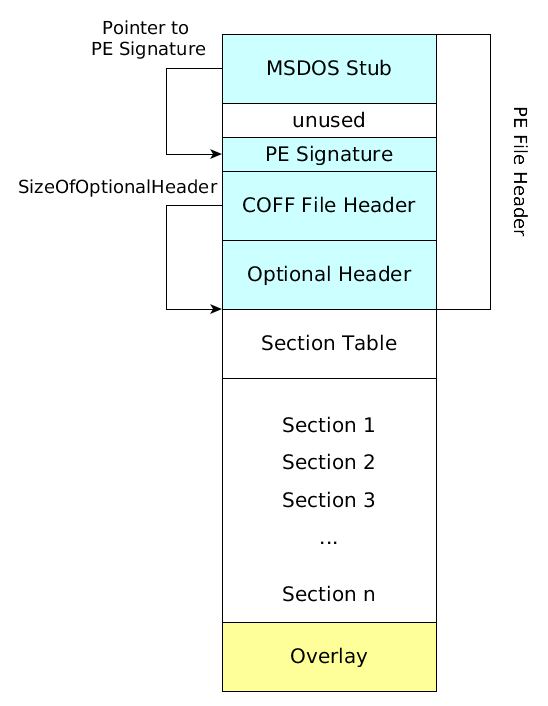
\includegraphics[width=.98\textwidth, height=\textheight,keepaspectratio]{graphics/peformat}
\caption{Structure of a PE file \protect{\cite{kath13}}}
\label{fig:peformat} 
\end{figure}

\section{Special Sections}

Sections may contain arbitrary information, which is only relevant to the application using them; but some sections have a special meaning. Their format is described in the PE COFF specification \cite{pespec}. These sections are recognized by entries in the Data Directory Table of the Optional Header. They have typical section names which are also used in the specification to refer to the sections. These names are not mandatory, but a convention. That's why they can not be relied on while trying to find certain sections.

Some of these special sections are described right after.

\subsection*{Import Section}

The import section contains data about the

\subsection*{Resource Section}

\subsection*{Debug Section}
